\documentclass{book}
\usepackage{listings}
\usepackage{hyperref}
\usepackage{verbatim}
\usepackage{amsmath}
\usepackage[backend=bibtex, sorting=none, style=numeric-comp, defernumbers]{biblatex}
\usepackage{graphicx}

\addbibresource{\jobname.bib}

\title{Chapter 3 - Unsupervised and Reinforcement learning}
\author{Joydeep Bhattacharjee}

\begin{document}
\maketitle

In the previous chapters we took a look at the regression and classification algorithms which fall under the category of Supervised algorithms\cite{UL:1} . In this chapter we will be taking a look at the remaining forms of machine learning, namely Unsupervised algorithms and reinforcement learning. In unsupervised algorithms the labels or the target classes are not given. So the goal of unsupervised learning is to attempt to find natural partitions of patterns. 

The main forms of performing unsupervised learning has been through clustering.

First we will focus on different unsupervised learning algorithms and how we can implement them using Rust. We will be using the same iris data set and the data preparation steps would be the same that we had seen in the chapter 2. Finally we should have two rusty machine dense matrices \lstinline{flower_x_train} and \lstinline{flower_x_test}. Although this data set is not totally conducive to unsupervised learning as we know the labels, yet this is a good data set for understanding the workings of creating unsupervised models.

\section{KMeans clustering}%
K-means is one of the simplest unsupervised learning algorithms that solve the clustering problem. The idea is to classify a data set through a certain number of clusters fixed apriori. If the number of clusters are k then the objective is to define k centers, one for each cluster. 

Commonly used initialization patterns for kmeans are Forgy, Random partition and KMeans++. The Forgy method randomly chooses k observations from the data set and uses them as the initial means. The random partition method first randomly assigns a cluster to each observation and then proceeds to the update step, thus computing the initial mean to be the centroid of the cluster's randomly assigned points. The Forgy method tends to spread the initial means out, while Random partition places all of them close to the center of the data set.

KMeans++ is almost the same as vanilla KMeans just that Kmeans++ starts with allocating one cluster center randomly and then searches for other centers given the first one\cite{UL:10}.

Using \lstinline{rusty-machine} we can use the \lstinline{KMeansClassifier} struct to implement apply KMeans on the data using the \lstinline{train} method. We can then either see the model centroids or run the predict method on the unseen data.

\begin{lstlisting}[caption={rusty\_machine\_unsupervised},basicstyle=\small]
use rusty_machine as rm;
use rm::learning::k_means::KMeansClassifier;

let mut model = KMeansClassifier::new(clusters);
model.train(&flower_x_train)?;
let centroids = model.centroids().as_ref().unwrap();
println!("Model Centroids:\n{:.3}", centroids);

println!("Predicting the samples...");
let classes = model.predict(&flower_x_test).unwrap();
println!("number of classes from kmeans: {:?}",
  classes.data().len());
\end{lstlisting}

Creating the above model initialises the k-means using kmeans$++$. Apart from this we can also use the Forgy or RandomPartition method.

\begin{lstlisting}[caption={rusty\_machine\_unsupervised},basicstyle=\small]
use rm::learning::k_means::{KMeansClassifier, Forgy,
                            RandomPartition, KPlusPlus};
// can use either Forgy or RandomPartition
let mut model = KMeansClassifier::new_specified(3, 100, Forgy);
\end{lstlisting}

where $3$ is the number of partitions and the number of epochs is kept at $100$.

\label{sec:kmeans_clustering}
\section{Gaussian Mixture Model}%
K-means and the associated expectation-maximization algorithm, is a special case of the Gaussian mixture model. The k-means clustering explored in the previous section is simple and relatively easy to understand, but its simplicity leads to practical challenges in its application. In particular, the non probabilistic nature of k-means and its use of simple distance-from-cluster-center to assign cluster membership leads to poor performance for many real world situations. In this section we will take a look at Gaussian Mixture Models (GMMs), which can be viewed as an extension of the ideas behind k-means, but can also be a powerful tool for estimation behind simple clustering \cite{UL:7} 

One way to think about the k-means model is that it places a circle sphere of influence (or a circle for the simplest case) at the center of each cluster, with a radius defined by the most distant points in the cluster. This radius acts as the hard cutoff for the cluster assignment within the training set: any point outside the circle is not considered a member of the cluster. A better model might be accounting for distributions where the distribution might be of a different shape. In GMMs the k-means is generalized to a probabilistic model where we assume that all the data points are generated from a mixture of a finite number of Gaussian distributions with unknown parameters.

\begin{figure}[htpb]
	\centering
	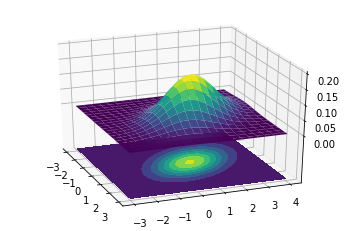
\includegraphics[width=0.8\linewidth]{gaussian_dist.png}
	\caption{Gaussian}
	\label{fig:gaussian}
\end{figure}

In the below picture we are using the iris dataset to map distribution between two variables \lstinline{sepal_length} and \lstinline{sepal_width}.

\begin{figure}[htpb]
	\centering
	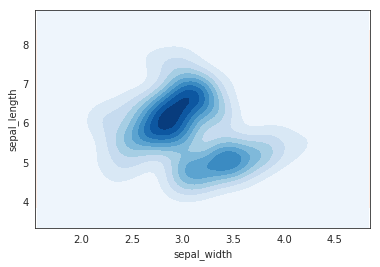
\includegraphics[width=0.8\linewidth]{multiple_contours.png}
	\caption{multiple distributions}
	\label{fig:multiple_distributions}
\end{figure}

A Gaussian distribution is completely determined by its covariance matrix and its mean. The covariance matrix of a Gaussian distribution determines the directions and lengths of the aces of its density contours, all of which are ellipsoids. The different type of covariance matrices are

\begin{itemize}
	\item \textbf{Full} means that the components may independently adopt any position and shape.
	\item \textbf{Tied} means they have the same shape but the shape may be anything.
	\item \textbf{Diagonal} means that the contour axes are oriented along the coordinate axes, but otherwise the eccentricities may vary between components.
	\item \textbf{Spherical} means that the contour is a sphere.
	\item \textbf{Toeplitz} means that the diagonals of the contour has elements that share the same paramters. It has an additional complexity parameter that selects the number of active off-diagonals and their constants.
	\item \textbf{Shrinked} means that the contour shape is determined by the complex combination of a diagonal and any covariance. No immediate obvious tying, but ties all eigenvalues so that they grow and shrink depending on the same parameter.
	\item \textbf{Kernel covariance}, in this case the covariance is defined by a positive definite function. We are in this case able to get a mixture model of functions (the greatest amount of generalisation mathematically speaking).
\end{itemize}

Apart from the above, constraints can be put on the Gaussian mixture composition, which increases generalisation of the model\cite{UL:8}.

Evaluation of the Gaussian Mixtures is done using the Expectation Maximisation algorithm. Expectation Maximisation is an iterative method to find maximum likelihood estimates of parameters in statistical models, where the model depends on unobserved latent variables. In this case we can think of the mixing probabilities of the Gaussian functions as the prior probabilities for the components. For given input values of the individual components, we can evaluate the corresponding posterior probabilities, called responsibilities. These responsibilities are essentially the latent variables\cite{UL:3} .

\paragraph{Rust}%
Using \lstinline{rusty-machine}, we can create a mixture model. Then we set the maximum number of iterations and the covariance types. We can then train this model using the \lstinline{train} method. Once training is done apart from the \lstinline{predict} method we will also be able to get the means and the covariances of the trained model and run the predict method.

\begin{lstlisting}[caption={rusty\_machine\_unsupervised},basicstyle=\small]
let mut model = GaussianMixtureModel::new(2);
model.set_max_iters(1000);
model.cov_option = CovOption::Diagonal;

println!("Training the model");
model.train(&flower_x_train)?;

// Print the means and covariances of the GMM
println!("{:?}", model.means());
println!("{:?}", model.covariances());

// Predict the classes and partition into
println!("Predicting the samples...");
let classes = model.predict(&flower_x_test).unwrap();
println!("number of classes from GMM: {:?}", classes.data().len());
\end{lstlisting}

In place of \lstinline{Diagonal}, we can also use the \lstinline{Full} and \lstinline{Regularized} options.`
\label{par:rust}


% http://ethen8181.github.io/machine-learning/clustering/GMM/GMM.html
% https://www.quora.com/When-learning-the-covariance-matrices-of-a-Gaussian-mixture-model-what-are-different-types-of-parameter-tying
% https://athemathmo.github.io/rusty-machine/doc/rusty_machine/learning/gmm/index.html
% http://www.cse.iitm.ac.in/~vplab/courses/DVP/PDF/gmm.pdf
% https://www.youtube.com/watch?v=JNlEIEwe-Cg
% http://statweb.stanford.edu/~tibs/stat315a/LECTURES/em.pdf

\label{sec:gaussian_mixture_model}

\section{Density Based Spatial Clustering of Applications with Noise}%
The DBSCAN algorithm views clusters as areas of high density separated by areas of low density. Due to this generic view, clusters found by DBSCAN can have any shape, as opposed to k-means which assumes that clusters are convex shape. Clusters are identified by looking at the density of points. Regions with a high density of points depict the existence of clusters whereas regions with a low density of points indicate clusters of noise or clusters of outliers. This algorithm is particularly suited to large data sets, with noise, and is able to identify clusters with different sizes and shapes.

The main concept of DBSCAN is that of core-samples, meaning that for each point of a cluster, the neighbourhood of a given radius has to contain atleast a minimum number of points, or in other words, the "density" in the neighbourhood has to exceed some predefined threshold. This algorithm needs three input parameters\cite{UL:9}.

\begin{itemize}
	\item k, the nearest neighbour list size.
	\item eps, the radius that delimit the neighbourhood area of a point.
	\item min points, the minimum number of points that must exist in the eps-neighbourhood.
\end{itemize}

The issues with DBSCAN is that it cannot handle varying densities. Also this algorithm is quite sensitive to parameters set.

DBSCAN models can be created using rusty-machine. In the below code we create a DBSCAN model with eps as $3$ and minimum samples as $10$. We then pass \lstinline{true} to \lstinline{set_predict} method of the model. This allows us to use the \lstinline{predict} on new unseen data. Similar to previous models we can train and predict on the data set. Apart from these we can also check the clusters which the model has learned.

\begin{lstlisting}[caption={rusty\_machine\_unsupervised},basicstyle=\small]
use rm::learning::dbscan::DBSCAN;
use rm::learning::UnSupModel;
let mut model = DBSCAN::new(0.3, 10);
model.set_predictive(true);

model.train(&flower_x_train)?;

let clustering = model.clusters().unwrap();

let classes = model.predict(&flower_x_test).unwrap();
\end{lstlisting}

Apart from \lstinline{DBSCAN::new} we can use \lstinline{DBSCAN::default}. The default values that are initialized are $0.5$ for eps, $5$ for minimum points.

\label{sec:dbscan}

\section{Principal Component Analysis}%
One of the main components of machine learning is matrix multiplication. Matrix multiplications are generally computationally expensive\cite{UL:4}. Also the number of dimensions that we are dealing with needs to be taken into account and we should not add too many dimensions unnecessarily. We are shown by the Hughes phenomenon that as the number of features increases, a classifiers performance increases as well until we reach the optimal number of features. Adding more features for the same size as the training set will degrade the features. This is called the curse of dimensionality\cite{UL:5}.

\begin{figure}[htpb]
	\centering
	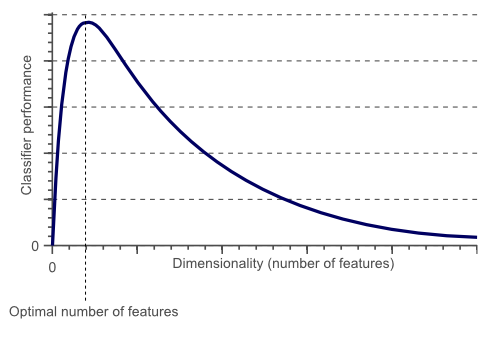
\includegraphics[width=0.8\linewidth]{HughesPhenomenon.png}
	\caption{Hughes Phenomenon}
	\label{fig:Hughes_Phenomenon}
\end{figure}

Many algorithms such as KNN are particularly susceptible to this curse of dimensionality. A way to escape this curse is by dimensionality reduction. In dimensionality reduction we generally choose a mathematical representation within which most of the variance in the original data, if not all, can be explained. The effect is that we are able to remove a significant number of features while retaining a lot of the information.

Principal Component Analysis is a method of dimensionality reduction. Its essentially a transformation where our original variables will get converted to a new set of variables, which are linear combinations of the original set of variables.

\begin{equation}
	PX = Y
\end{equation}

where X is the original recorded data set, Y is the representation of the data set and P is the linear transformation matrix. Geometrically we can see that P is a rotation and stretch from $X$ to $Y$. 
\label{par:singular_value_decomposition}

\paragraph{PCA and Rust}%
Although PCA has been implemented in \lstinline{rusty-machine}, it has not been published in the crate as of the writing of this book. Hence we will need to update the dependencies in Cargo.toml file to pull in the latest code from the master

\begin{lstlisting}[caption={Cargo.toml},basicstyle=\small]
[dependencies]
rusty-machine = { git = "https://github.com/AtheMathmo/rusty-machine.git", rev = "f43da8d" }
\end{lstlisting}

Now we should be able to create a PCA model and train on the data. In this case we are reducing the dimensions to 2 and ask the model to center the clusters.

\begin{lstlisting}[caption={rusty\_machine\_unsupervised},basicstyle=\small]
use rm::learning::pca::PCA;
use rm::learning::UnSupModel;
let mut model = PCA::new(2, true);
model.train(&flower_x_train)?;

println!("{:?}", model.predict(&flower_x_test)?);
println!("{:?}", model.components());
\end{lstlisting}

We can also use the \lstinline{PCA::default} method to create a default model, but the default model has all the components. So we will not be having reduction in the dimensions then.

\label{par:pca_and_rust}

% https://www.cs.cmu.edu/~elaw/papers/pca.pdf

\label{sec:principal_component_analysis}

\section{Testing an Unsupervised model}%
Evaluating the performance of an unsupervised model is difficult as there are no labels to compare the final score with. One way is through internal metrics such as the silhouette score, which aims at formalizing the attainment of high intra-cluster similarity, or points within a cluster should be close to each other and low inter-cluster similarity which means similarity between points in two clusters should be low. But good scores on an internal criterion may not necessarily translate into good effectiveness in application. The other approach is through direct evaluation in the application of interest. For example a website implementing search may measure the time taken by the users to find an answer with different clustering algorithms and the two algorithms can be compared with beta testing. This is the most direct evaluation, but it is expensive, especially if large user studies are necessary.

A third approach by using a surrogate of user judgements, in which case we use a set of classes and create a gold standard ourselves. The gold standard is ideally produced by human judges with good level of inter-judge agreement. We can then compute an external criterion that evaluates how well the cluster matches the gold standard classes. In this section two measures of external criteria are described with code accompanying them.

\paragraph{Rand Index}%
The Rand Index computes a similarity measure between two clusterings by considering all pairs of samples and counting pairs that are assigned in the same or different clusters in the predicted and true clusterings. The most common formulation of he Rand index focuses on the following four sets of the $\binom nk$ element pairs:: $N_{11}$ is the number of element pairs that are grouped in the same cluster in both clusterings, $N_{10}$ is the number of element pairs which are grouped in the same cluster by $A$ but in different clusters by $B$, $N_{01}$ the number of element pairs which are grouped in the same cluster by $B$ but in different clusters by $A$, and $N_{00}$ the number of elements pairs which are grouped in different clusters by both $A$ and $B$. Notice that $N_{11}$ and $N_{00}$ are the indicator of agreements between clusters $A$ and $B$ while $N_{10}$ and $N_{01}$ are the disagreements.

\begin{table}[htpb]
	\centering
	\caption{contingency table}
	\label{tab:label}
	\begin{tabular}{|l|l|l|l|l|l|}
            $A$/$B$ & $B_1$    & $B_2$    & \dots  & $B_n$    & Sums  \\ \hline
            $A_1$   & $n_{11}$ & $n_{12}$ & \dots  & $n_{1n}$ & $a_1$ \\
            $A_2$   & $n_{21}$ & $n_{22}$ & \dots  & $n_{2n}$ & $a_2$ \\
            $\vdots$  & $\vdots$   & $\vdots$   & $\vdots$ & $\vdots$   & $\vdots$ \\
            $A_n$   & $n_{n1}$ & $n_{n2}$ & $\ddots$ & $n_{nn}$ & $a_n$ \\ \hline
            Sums    & $b_1$    & $b_2$    & $\dots$  & $b_n$    & $N$
	\end{tabular}
\end{table}

The contingency is shown in table 1. Therefore the rand index would be given by the below function

\begin{equation}
	RI(A, B) = \frac{N_{11} + N_{00}}{\binom nk}
\end{equation}

The value of the above index would lie between 0 and 1, where 1 indicates that the clusterings are identical and 0 means that the clusters do not share a single pair of elements.

Rand index is implemented in \lstinline{ml-utils}.

\begin{lstlisting}[caption={ml\\-utils\\/src\\/unsup\_metrics\\.rs},basicstyle=\small]
pub fn rand_index(clusters1: &[HashSet<u64>],
    clusters2: &[HashSet<u64>]) -> f64 {
  let (n11, n10, n01, n00) = count_pairwise_cooccurence(
    clusters1, clusters2);
  (n11 + n00) / (n11 + n10 + n01 + n00)
}
\end{lstlisting}

The implementation of \lstinline{count_pairwise_cooccurence} function can be found on the same module and has been skipped for brevity.

We should now be able to run this function and get the index.

\begin{lstlisting}[caption={ml\\-utils\\/src\\/unsup\_metrics\\.rs},basicstyle=\small]
use ml_utils::unsup_metrics::rand_index;

println!("rand index: {:?}",
  rand_index(&predicted_clusters, &flower_y_test_clus));
\end{lstlisting}

\label{par:rand_index}

\paragraph{Jaccard Index}%
Similar to the rand index we have the jaccard index. It is defined by the size of the intersection divided by the size of the union.

\begin{equation}
	J(A, B) = \frac{|A \cap B|}{|A \cup B|}
\end{equation}

This can be easily understood by the figure: 4. The intersection should approach the union as the clusters are similar to each other.

\begin{figure}[]
	\centering
	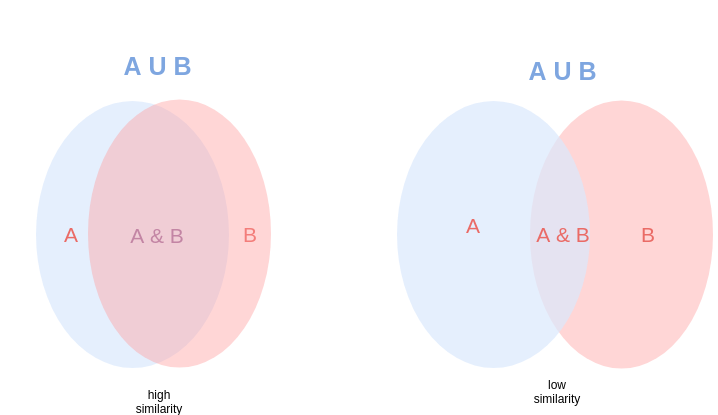
\includegraphics[width=0.8\linewidth]{jaccard.png}
	\caption{Jaccard}
	\label{fig:jaccard}
\end{figure}

Take a look at the implementation of jaccard index in \lstinline{ml-utils}.

\begin{lstlisting}[caption={ml\\-utils\\/src\\/unsup\_metrics\\.rs},basicstyle=\small]
pub fn jaccard_index(clusters1: &[HashSet<u64>],
    clusters2: &[HashSet<u64>]) -> f64 {
  let (n11, n10, n01, n00) = count_pairwise_cooccurence(clusters1, clusters2);
  let denominator = n11 + n10 + n01;
  if denominator > 0.0 {
    return n11 / denominator;
  } else {
    0.0
  }
}
\end{lstlisting}

We should now be able to run this function and get the index.

\begin{lstlisting}[caption={ml\\-utils\\/src\\/unsup\_metrics\\.rs},basicstyle=\small]
use ml_utils::unsup_metrics::jaccard_index;

println!("jaccard index: {:?}",
  jaccard_index(&predicted_clusters, &flower_y_test_clus));
\end{lstlisting}

\label{par:jaccard_index}

% https://medium.com/hockey-stick/tl-dr-bayesian-a-b-testing-with-python-c495d375db4d
% https://towardsdatascience.com/the-math-behind-a-b-testing-with-example-code-part-1-of-2-7be752e1d06f
% https://nlp.stanford.edu/IR-book/html/htmledition/evaluation-of-clustering-1.html
% find ways to give similarity scores https://github.com/Hoosier-Clusters/clusim/tree/master/clusim

\label{sec:testing_an_unsupervised_model}

\section{Reinforcement learning}%
Reinforcement learning is the utilisation of different algorithms so that a suitable action can be chosen to maximise reward in a given situation. The difference from supervised learning is that the labeled input/output pairs may not be present. In unsupervised learning, we are interested in finding the similarities and differences between the data points. But reinforcement learning is more about finding the best behaviour given an environment. To build a reinforcement system, the software system should have a mechanism to make observations and take actions within an environment. In return it should recieve rewards in some form. The idea is to maximise long term rewards.

The algorithm that is used by the software to determine its actions is called its policy. The policy should have access to two functions of the target body, a way to take observations as inputs and a way to take the next step.

One of the challenges of reinforcement learning is that in order to train an agent we need to create the environment. The environment can be both real world and software simulations. Real world simulations are outside the scope of this book so we will target a subset of software simulations. One of the great crates for reinforcement learning is \lstinline{rsrl}. Since the current changes have not been pushed to the crate we will use the git master as dependency. Creating custom crates also involve a little bit of internal objects and hence we will be using a slightly modified version in the code.


\begin{lstlisting}[caption={chapter3\\/rsrl\_custom\\/Cargo\\.toml},basicstyle=\small]
[dependencies]
rsrl = { git = "https://github.com/infinite-Joy/rsrl", branch = "mymodel" }
slog = "2.4.1"
ndarray = "0.12.0"
\end{lstlisting}

Now we should be able to create a custom model. Most of the code here has been taken from the A2C examples and the Cartpole problem in reinforcement learning. The cartpole problem also known as the inverted pendulum is a pendulum with the center of gravity above the pivot point. This results in the pendulum being very unstable. The goal is to keep the pole balanced by applying forces in the appropriate direction at the pivot point.

\begin{figure}
\begin{center}
	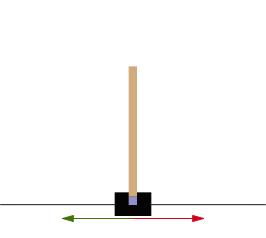
\includegraphics[scale=0.6]{Figures/cartpole.png}
\end{center}
\caption{}
\label{fig:cartpole}
\end{figure}

At each time step we are able to observe its position $x$, velocity $dx$, angle $\theta$ and angular velocity $d\theta$. Thus the state-space has four dimensions of continuous values and the action space has one dimension of two discrete values. The force can be represented by \lstinline{ALL_ACTIONS}.


\begin{lstlisting}[caption={chapter3\\/rsrl\_custom\\/src\\/main\\.rs},basicstyle=\small]
const ALL_ACTIONS: [f64; 2] = [-1.0 * CART_FORCE, 1.0 * CART_FORCE];
\end{lstlisting}

And we will need to define the environment by the scope of the current state and what will happen when a force is applied.

\begin{lstlisting}[caption={chapter3\\/rsrl\_custom\\/src\\/main\\.toml},basicstyle=\small]
impl CartPole {
  fn new(x: f64, dx: f64, theta: f64, dtheta: f64) -> CartPole {
    CartPole {
      state: Vector::from_vec(vec![x, dx, theta, dtheta]),
    }
  }

  fn update_state(&mut self, a: usize) {
    let fx = |_x, y| CartPole::grad(
      ALL_ACTIONS[a], &y); // when a force <a> is applied
    let mut ns = runge_kutta4(
      &fx, 0.0, self.state.clone(), TAU);

    ns[StateIndex::X] = clip!(
      LIMITS_X.0, ns[StateIndex::X], LIMITS_X.1);
    ns[StateIndex::DX] = clip!(
      LIMITS_DX.0, ns[StateIndex::DX], LIMITS_DX.1);

    ns[StateIndex::THETA] = clip!(
      LIMITS_THETA.0, ns[StateIndex::THETA], LIMITS_THETA.1);
    ns[StateIndex::DTHETA] = clip!(
      LIMITS_DTHETA.0, ns[StateIndex::DTHETA], LIMITS_DTHETA.1);

    self.state = ns;
  }

  fn grad(force: f64, state: &Vector) -> Vector {
    let dx = state[StateIndex::DX];
    let theta = state[StateIndex::THETA];
    let dtheta = state[StateIndex::DTHETA];

    let cos_theta = theta.cos();
    let sin_theta = theta.sin();

    let z = (force
             + POLE_MOMENT
	     * dtheta * dtheta
	     * sin_theta) / TOTAL_MASS;

    let numer = G * sin_theta - cos_theta * z;
    let denom = FOUR_THIRDS
      * POLE_COM
      - POLE_MOMENT
      * cos_theta * cos_theta;

    let ddtheta = numer / denom;
    let ddx = z - POLE_COM * ddtheta * cos_theta;

    Vector::from_vec(vec![dx, ddx, dtheta, ddtheta])
  }
}
\end{lstlisting}

In rsrl to implement this environment, we will need to implement the Domain trait. If we see the signature of the Domain trait we get an understanding of the types of behavior that we need to implement. This can be seen in \href{}{https://github.com/tspooner/rsrl/blob/master/src/domains/mod.rs}


\begin{lstlisting}[caption={},basicstyle=\small]
pub trait Domain {
    type StateSpace: Space;
    type ActionSpace: Space;
    fn emit(&self) -> .. // this is for observation
    fn step( .. // given an action what should be the next state.
    fn is_terminal(&self) -> bool; // this is to end the sequence of action sometime.
    fn reward( .. // a reward mechanism
    fn state_space(.. // returns an instance of state space
    fn action_space(.. // returns an instance of the action class.
}
\end{lstlisting}

Coming back to Cartpole first we define a default.

\begin{lstlisting}[caption={chapter3\\/rsrl\_custom\\/src\\/main\\.rs},basicstyle=\small]
impl Default for CartPole {
  fn default() -> CartPole { CartPole::new(0.0, 0.0, 0.0, 0.0) }
}
\end{lstlisting}

Now we should be able to implement the Domain behaviors for Cartpole. We first define the state space and the action space.

\begin{lstlisting}[caption={chapter3\\/rsrl\_custom\\/src\\/main\\.rs},basicstyle=\small]
impl Domain for CartPole {
  type StateSpace = LinearSpace<Interval>;
  type ActionSpace = Ordinal;
\end{lstlisting}

\lstinline{emit} is simple. If its the last state then we define it as terminal else we define it as full.

\begin{lstlisting}[caption={chapter3\\/rsrl\_custom\\/src\\/main\\.rs},basicstyle=\small]
impl Domain for CartPole {
  // code ..

  fn emit(&self) -> Observation<Vector<f64>> {
    if self.is_terminal() {
      Observation::Terminal(self.state.clone())
    } else {
      Observation::Full(self.state.clone())
    }
  }

  fn is_terminal(&self) -> bool {
    let x = self.state[StateIndex::X];
    let theta = self.state[StateIndex::THETA];

    x <= LIMITS_X.0
      || x >= LIMITS_X.1
      || theta <= LIMITS_THETA.0
      || theta >= LIMITS_THETA.1
  }
\end{lstlisting}

Now we will need to implement behaviors for \lstinline{reward} and \lstinline{state_space}.

\begin{lstlisting}[caption={chapter3\\/rsrl\_custom\\/src\\/main\\.rs},basicstyle=\small]
fn reward(&self, _: &Observation<Vector<f64>>, to: &Observation<Vector<f64>>) -> f64 {
  match *to {
    Observation::Terminal(_) => REWARD_TERMINAL,
    _ => REWARD_STEP,
  }
}

fn state_space(&self) -> Self::StateSpace {
  LinearSpace::empty() + Interval::bounded(LIMITS_X.0, LIMITS_X.1)
    + Interval::bounded(LIMITS_DX.0, LIMITS_DX.1)
    + Interval::bounded(LIMITS_THETA.0, LIMITS_THETA.1)
    + Interval::bounded(LIMITS_DTHETA.0, LIMITS_DTHETA.1)
}

fn action_space(&self) -> Ordinal { Ordinal::new(2) }
\end{lstlisting}

Currently there are different reinforcement algorithms that can be used to train the environment. We have the actor critic system, doing this using Q-learning, with some variants. In the example we have taken the actor critic system. The idea behind them is simple. There are essentially two systems that needs to be trained. One is the critic that measures how good the action taken is and the actor that controls how the agent behaves. So we will need to first define the agent and the critic.

\begin{lstlisting}[caption={chapter3\\/rsrl\_custom\\/src\\/main\\.rs},basicstyle=\small]
fn main() {
  let domain = CartPole::default();

  let n_actions = domain.action_space().card().into();
  let bases = Fourier::from_space(
    3, domain.state_space()).with_constant();

  let policy = make_shared({
    let fa = LFA::vector(bases.clone(), n_actions);

    Gibbs::new(fa)
  });
  let critic = {
    let q_func = LFA::vector(bases, n_actions);

    SARSA::new(q_func, policy.clone(), 0.1, 0.99)
  };

let mut agent = A2C::new(critic, policy, 0.01);
// rest of the code ..
\end{lstlisting}

Once they are created, we can go ahead and train to system to finding the optimal policy. In this case we can go through 1000 episodes to get the optimal policy.

\begin{lstlisting}[caption={chapter3\\/rsrl\_custom\\/src\\/main\\.rs},basicstyle=\small]
let logger = logging::root(logging::stdout());
let domain_builder = Box::new(CartPole::default);

let _training_result = {
  let e = SerialExperiment::new(&mut agent, domain_builder.clone(), 1000);
  run(e, 1000, Some(logger.clone()))
};

let testing_result = Evaluation::new(
  &mut agent, domain_builder).next().unwrap();

info!(logger, "solution"; testing_result);
\end{lstlisting}

Running this would return the number of steps that are required.

\label{sec:Reinforcement learning}


\section{Conclusion}%
In this chapter we explored unsupervised learning and reinforcement learning. In unsupervised learning we looked at how to implement Kmeans, gaussian mixture models and DBSCAN for clustering and PCA for dimensionality reduction using rusty-machine using a dataset without labels. Then we looked at evaluation clustering models using two popular methods the rand index and the jaccard index. The basic methods of implementing other evaluation criteria would be similar.

Lastly we explored reinforcement learning and how to implement a custom model using in rsrl.

In the next chapter we will be moving away from models and focusing on another important dimension of machine learning, which is how to work with common data storage technologies and formats, we will also learn how to create structured data if the data available is not structured at all.
\label{sec:conclusion}

\printbibliography
\nocite{*}
\end{document}
